\chapter{Desenvolvimento de Projetos com o AndroMDA}

Nesta seção veremos os passos necessários ao desenvolvimento de projetos com o MDArte, utilizando os cartuchos EJB, Hibernate e BPM4Struts.

\section{Criação de um Novo Projeto e Configuração do ambiente}

O plugin do MDArte para o Maven já possui um procedimento parametrizado para criação de projetos, que funciona como um wizard, onde o usuário deve responder a perguntas. Através das respostas fornecidas, o MDArte direcionará a criação da estrutura básica e dos artefatos básicos de configuração de projetos. O procedimento para criação de um novo projeto é:

\begin{enumerate}
\item Abra o terminal (command prompt) e vá para o diretório onde se deseja
criar o projeto. Na verdade, o projeto será gerado em um subdiretório do diretório escolhido. No Windows, não se pode ter espaços em branco no caminho desse diretório. Exemplo de diretório inválido:

C:$\backslash$Documents and Settings$\backslash$MDArte.

\item Digite o comando: maven andromdapp:generate

\item Responda as perguntas de acordo com o seu projeto. Abaixo um exemplo com respostas típicas (perguntas em negrito):

\textbf{Please enter your first and last name (i.e. Rodrigo Salvador):} \\
MDArte\\
\textbf{Please enter the name of your J2EE project (i.e. Sistema Academico):}\\
Sistema Academico\\
\textbf{Please enter the id for your J2EE project (i.e. sistemaacademico):}\\
sistemaacademico\\
\textbf{Please enter a version for your project (i.e. 1.0):}\\
1.0\\
\textbf{Please enter the base package name for your J2EE project (i.e. br.mdarte.exemplo.academico):}\\
br.mdarte.exemplo.academico\\
\textbf{Would you like to enable security? (enter 'yes' or 'no')?}\\
yes\\
\textbf{Would you like to use oAuth (enter 'yes' or 'no') ?}\\
no\\
\textbf{Would you like to use MDArte's default Controle Acesso (enter 'yes' or
'no') ?}\\
yes\\
\textbf{Would you like to use modules (enter 'yes' or 'no')?}\\
yes\\
\textbf{Please enter the EJB version number (enter '2' or '3'):}\\
3\\
\textbf{Please enter the Struts version number (enter '1' or '2'):}\\
2\\
\textbf{Would you like to enable the JUnit support for general testing? (enter
'yes' or 'no')? }\\
 no\\
\textbf{Please enter the database backend for the persistence layer: (enter
'hypersonic' or 'mysql' or 'oracle' or 'postgres')}\\
 postgres\\
 
\item Após receber as respostas, o MDArte criará um subdiretório onde será gerada a estrutura inicial do projeto. A partir desse momento chamaremos esse diretório de <DiretorioProjeto>.

\item Ainda no console, vá para o diretório onde está seu projeto: <DiretorioProjeto>.

\item Digite maven. Isto obrigará o Maven a obter todos os artefatos (por exemplo, bibliotecas) de que o projeto dependerá.

\end{enumerate}

\section{Configuração do Banco}
Para se configurar o Banco de Dados é necessário modificar o arquivo project.properties da raiz do projeto, onde se encontram as propriedades que devem ser alteradas. Abaixo estão as propriedades do arquivo de configuração para cada um dos Bancos de Dados

\begin{itemize}
	\item [Oracle] \hfill
	\begin{itemize}
		\item dataSource.driver.jar=\textdollar{}\{env.JBOSS\_HOME\}/server/default/lib/ojdbc14.jar
		\item dataSource.driver.class=oracle.jdbc.driver.OracleDriver
		\item sql.mappings=Oracle9i
		\item hibernate.db.dialect=org.hibernate.dialect.Oracle9Dialect
	\end{itemize}
	\item [SQLServer] \hfill
	\begin{itemize}
		\item dataSource.driver.jar=\textdollar{}\{env.JBOSS\_HOME\}/server/default/lib/jtds-1.1.jar
		\item dataSource.driver.class=net.sourceforge.jtds.jdbc.Driver
		\item sql.mappings=MSSQL
		\item hibernate.db.dialect=org.hibernate.dialect.SQLServerDialect
	\end{itemize} 
	\item [Postgres] \hfill
	\begin{itemize}
		\item dataSource.driver.jar=\textdollar{}\{env.JBOSS\_HOME\}/server/default/lib/postgresql-8.1-405.jdbc3.jar
		\item dataSource.driver.class=org.postgresql.Driver
		\item defaultHibernateGeneratorClass=sequence
		\item sql.mappings=PostgreSQL
		\item hibernate.db.dialect=PostgreSQLDialect
	\end{itemize}
	\item [MySQL] \hfill
	\begin{itemize}
		\item dataSource.driver.jar=\textdollar{}\{env.JBOSS\_HOME\}/server/default/lib/mysql-connector-java-5.1.6-bin.jar
		\item dataSource.driver.class=com.mysql.jdbc.Driver
		\item defaultHibernateGeneratorClass=native
		\item sql.mappings=MySQL
		\item hibernate.db.dialect=org.hibernate.dialect.MySQLDialect
	\end{itemize}
\end{itemize}

Outro arquivo que deve ser alterado ou criado é o arquivo de configurações do Banco de Dados do JBoss, localizado no diretório JBOSS\_HOME/server/default/deploy/, com formação do nome terminando com -ds.xml (ex.: aplicacoes-ds.xml), que deve ter a tag <local-tx-datasource> preenchida de acordo com as informações fornecidas no arquivo <projeto>/project.properties.

Exemplo (usando banco Postgres):

\begin{lstlisting}[language=xml]
<local-tx-datasource>
	<jndi-name>sistemaacademicoDS</jndi-name>
	<use-java-context>true</use-java-context>
	<connection-url>
		jdbc:postgresql://127.0.0.1:5432/sistemaacademico
	</connection-url> 
	<driver-class>org.postgresql.Driver</driver-class>
		<user-name>usuario</user-name>
		<password>senha</password>
<!--
	<exception-sorter-class-name>
		org.jboss.resource.adapter.jdbc.vendor.OracleExceptionSorter
	</exception-sorter-class-name>
-->
	</local-tx-datasource>
\end{lstlisting}

Repare que no exemplo anterior, o nome do Data Source é sistemaacademicoDS, que deve ser o mesmo nome informado no arquivo project.properties da raiz do projetom ou seja `sistemaacademicoDS`.

Além disso, o arquivo login-config.xml, localizado no diretório JBOSS\_HOME/server/default/conf/, deverá ser modificado, adicionando-se a ele o seguinte trecho:

\begin{lstlisting}[language=xml]
<!--
SistemaAcademico Policy
-->
<application-policy name="sistemaacademico">
	<authentication>
		<login-module code="org.jboss.security.ClientLoginModule"
			flag="required">
			<module-option name="multi-threaded">true
				</module-option>
		</login-module>
		<login-module code="accessControl.LoginModuleImpl" 
			flag="required">
			<module-option name="dsJndiName">java:/controleacessoDS
				</module-option>
			<module-option name="unauthenticatedIdentity">guest
				</module-option>
			<module-option name="principalClass">
				accessControl.PrincipalImpl</module-option> 
			<module-option name="hashEncoding">hex</module-option> 
			<module-option name="hashAlgorithm">md5</module-option>
			<module-option name="principalsQuery">
				select SENHA from OP_C_A where LOGIN=?
				</module-option>
			<module-option name="rolesQuery">
				select OP_PF.PF_OP_C_A_FK, 'Roles'
				12from OP_C_A, OP_C_A_PF_OP_C_A OP_PF
				where LOGIN=? AND OP_C_A.ID = OP_PF.OP_C_A_FK
			</module-option>
		</login-module>
	</authentication>
</application-policy>
\end{lstlisting}

As informações presentem nesse arquivo permitirão a aplicação do Sistema Acadêmico se conectar a base de dados e validar o usuário no momento de login.

\section{Controle de Acesso}

Neste tutorial estaremos utilizando funcionalidades de controle de acesso, porém não é nosso propósito explorar suas funcionalidades. Assim, estaremos utilizando um projeto de controle de acesso desenvolvido pela comunidade do MDArte.

O projeto pode ser obtido a partir do repositório Git do MDArte, pelo endereço https://github.com/MDArte/controleacesso.git . Por fim, edite também o arquivo project.properties do ControleAcesso para configurar o tipo de Banco de Dados a ser utilziado, conforme realizado com o projeto SistemaAcademico. Note que a propriedade dataSource.name está definida como ControleAcessoDS.

Novamente, precisaremos criar um arquivo de configuração do Banco de Dados, localizado no diretório JBOSS\_HOME/server/default/deploy/ . O nome do arquivo deve seguir a mesma formatação mencionada, terminando em -ds.xml (ex.: aplicacoes-ds.xml), podendo estar no mesmo arquivo com as configurações do projeto SistemaAcademico.

Exemplo:

\begin{lstlisting}[language=xml]
<local-tx-datasource>
	<jndi-name>controleacessoDS</jndi-name>
	<use-java-context>true</use-java-context>
	<connection-url>jdbc:postgresql://127.0.0.1:5432/controleacesso
		</connection-url> 
	<driver-class>org.postgresql.Driver</driver-class>
	<user-name>usuario</user-name>
	<password>senha</password>
	<!--<exception-sorter-class-name>
	org.jboss.resource.adapter.jdbc.vendor.OracleExceptionSorter
	</exception-sorter-class-name>-->
</local-tx-datasource>
\end{lstlisting}

Note que no exemplo anterior o ControleAcesso estará utilizando a mesma base de dados do projeto SistemaAcademico, definida pela tag <connection-url>. Agora, execute os seguinte comandos, na raiz do projeto ControleAcesso, para gerar, compilar e copiar os pacotes para o diretório JBOSS\_HOME/server/default/deploy/:

\begin{lstlisting}[language=bash]
maven mda -Dprojeto=ca-core
cd common
maven jar:install deploy
cd ../core/cd
maven jar:install deploy
\end{lstlisting}

\section{Modelando o nosso primeiro projeto}

Nesta seção iremos modelar um exemplo de Sistema Acadêmico básico, mostrando o quão rápido e simples pode ser usar o MDArte e todo o seu poder de geração.

Para esta parte do tutorial usaremos o MagicDraw. Na barra de ferramentas do MagicDraw, clicaremos em 'Open Project' e abriremos o xml do projeto, SistemaAcademico.xml no caminho <DiretorioProjeto>/mda/src/uml/.

\subsection{Modelando a camada de domínio}
Na camada de domínio, estarão as classes do domínio da aplicação. Elas serão entidades e estarão associadas a algum modo de persistência. Essas classes deverão conter o estereótipo «Entity» e os atributos que serão persistidos. Todas as classes de entidade devem obrigatoriamente estar no pacote <PacoteProjeto>.cd, em que <PacoteProjeto> é o pacote definido para o projeto.

Atualmente, estamos utilizando framework Hibernate para esta camada. 

Neste exemplo, especificamente, iremos também marcar nossas entidades com o estereótipo «Manageable», tal marcação diz para o MDArte que desejamos que seja gerado um CRUD padrão para tais entidades, sem a necessidade de modelarmos o mesmo diretamente.

\begin{enumerate}
\item Crie a mesma estrutura de pacotes que foi definida na criação do projeto.
Dentro da estrutura, crie o pacote “cd”.
\begin{figure}[!htb]
	\centering
	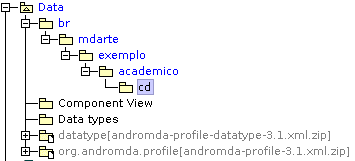
\includegraphics[width=250pt,height=100pt]{imgs/tutorial-mdarte-0000.png}
\end{figure}
\item Clique com o botão direito do mouse no pacote “cd” e selecione a opção New
Diagram.Em seguida, selecione Class Diagram.
\begin{figure}[!htb]
	\centering
	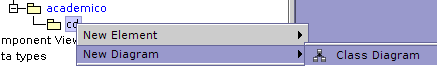
\includegraphics[width=400pt,height=60pt]{imgs/tutorial-mdarte-0001.png}
\end{figure}
	
\item Indique o nome desejado para diagrama (ex: Entidades).
	
\item No diagrama de classe, crie uma nova classe. Clique com o botão direto sobre a classe e selecione a opção Specification. Defina o nome da classe como “Estudante”.
	
\item Crie os atributos na classe Estudante (matricula, nome) selecionando a aba Attributes e clicando no botão Add. A figura abaixo exemplifica a criação do atributo matricula. O campo Visibility deve ser public. Não é necessário modelar o atributo id, pois ele é gerado automaticamente. Como mostra a Figura~\ref{config_parametro}.

\begin{figure}[!htb]
	\centering
	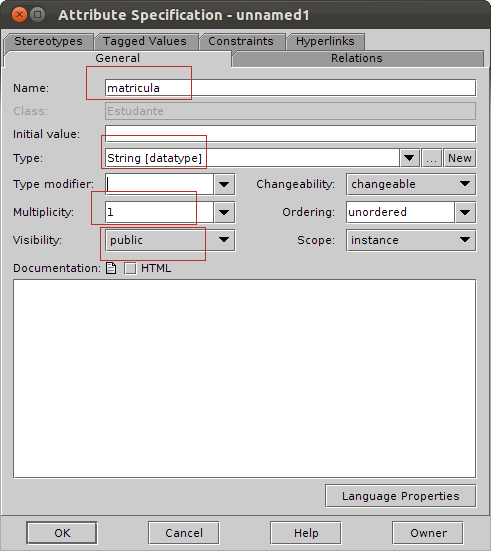
\includegraphics[width=350pt,height=400pt]{imgs/tutorial-mdarte-0002.png}
	\caption{Configuração do parâmetro matrícula da classe Estudante.}
	\label{config_parametro}
\end{figure}
		
A multiplicidade com valor 1 (campo Multiplicity) indica que o atributo é obrigatório (NOT NULL), já o valor 0..1 indica que o atributo não é obrigatório. Por padrão, todos os atributos são gerados como NOT NULL.

\item Coloque o estereótipo «Unique» no atributo matricula para indicar que cada código deve ser único, ou seja, não pode haver duas matrículas iguais. Abra a especificação do atributo matricula e selecione a aba Stereotypes. Nessa aba selecione o estereótipo «Unique».

\begin{figure}[!htb]
	\centering
	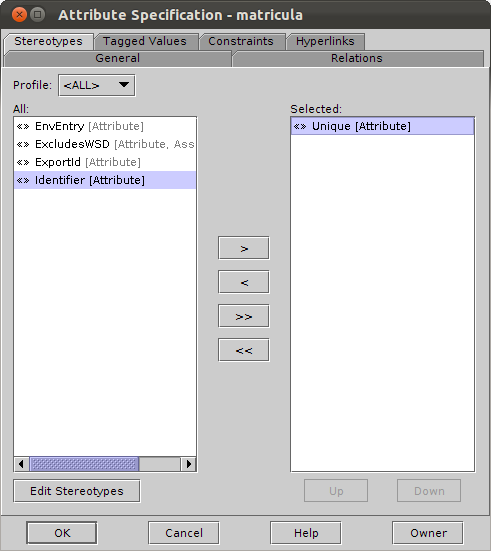
\includegraphics[width=350pt,height=400pt]{imgs/tutorial-mdarte-0003.png}
\end{figure}
	
\item Coloque os estereótipos «Entity» e «Manageable» na classe Estudante.
\begin{figure}[!htb]
	\centering
	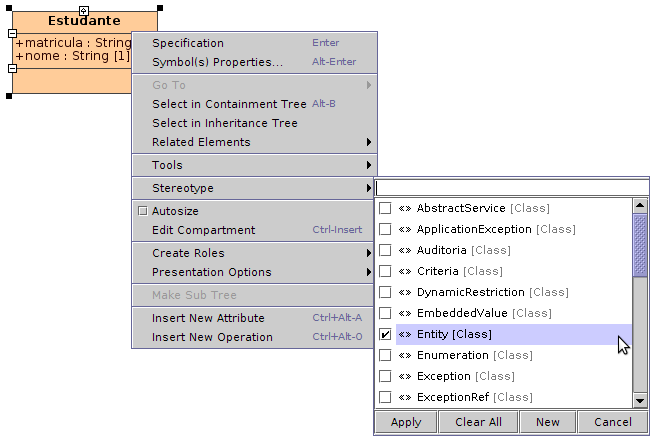
\includegraphics[width=400pt,height=300pt]{imgs/tutorial-mdarte-0004.png}
\end{figure}
	
Para cada entidade, também podem ser atribuídos valores etiquetados para agregar ao modelo parâmetros para a geração de código. Por exemplo, o valor etiquetado @andromda.persistence.table reflete o nome da tabela a ser criada no Banco de Dados. Da mesma forma, podemos atribuir estereótipos e valores etiquetados aos atributos. Entre os estereótipos temos: «Identifier» que determina que o atributo será o identificador do objeto (possível chave primária) e «Entity» que determina que o valor do atributo deverá ser único.

Como exemplo de valores etiquetados temos @andromda.persistence.column que define o nome da coluna a ser criada no Banco de Dados e @andromda.persistence.column.lenght que define o tamanho da coluna.

\item No mesmo diagrama de classes, crie outra classe. Clique com o botão direto sobre a classe e selecione a opção Specification. Defina o nome da classe como “Curso”.
	
\item Crie os atributos na classe Curso (codigo, nome) selecionando a aba Attributes e clicando no botão Add. O campo Visibility deve ser public, assim como feito anteriormente.

\item Coloque o estereótipo «Unique» no atributo codigo para indicar que cada código deve ser único. Abra a especificação do atributo codigo e selecione a aba Stereotypes. Nessa aba selecione o estereótipo «Unique».
	
\item Coloque o estereótipo «Entity» na classe.
	
\item Agora, crie uma associação entre as classes. Vá no diagrama de classes e puxe uma relação Association de uma classe para outra.
	
\item A associação será de 1 para muitos. Assim, clique duas vezes na associação e irá aparecer a tela de especificação. Edite os campos Multiplicity definindo valor “0..*” para a entidade Estudante e “1” para a entidade Curso.

\begin{figure}[!htb]
	\centering
	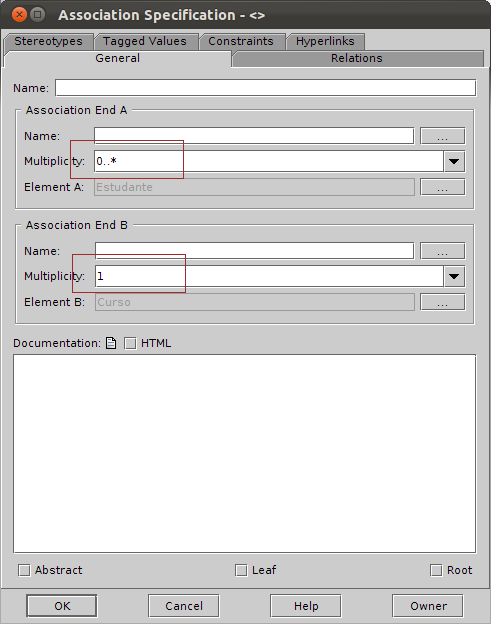
\includegraphics[width=350pt,height=400pt]{imgs/tutorial-mdarte-0005.png}
\end{figure}
	
\item A associação deve ser dupla, tanto Estudante quanto Curso devem ser visíveis. Dessa forma, mantenha a checkbox Navigable marcada na associação para as duas classes. Para isso, clique no botão “...” (reticências) da tela anterior.

\begin{figure}[!htb]
	\centering
	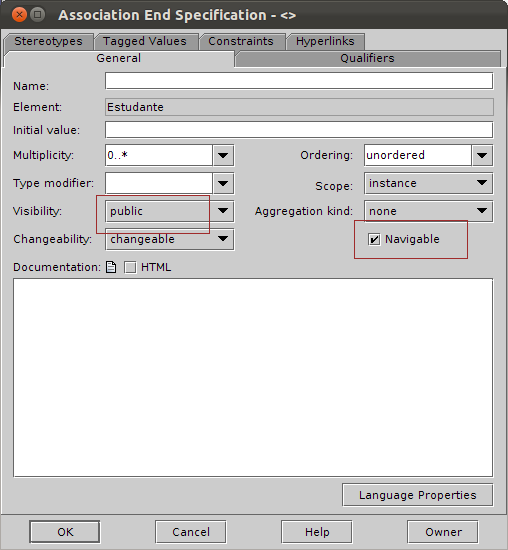
\includegraphics[width=350pt,height=400pt]{imgs/tutorial-mdarte-0006.png}
\end{figure}
		
O resultado final será: \hfill
\begin{figure}[!htb]
	\centering
	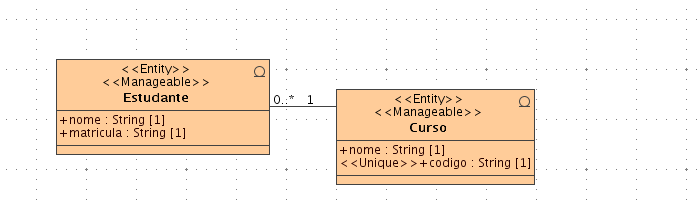
\includegraphics[width=500pt,height=200pt]{imgs/tutorial-mdarte-0007.png}
\end{figure}
	
\item No diretório da aplicação, execute o comando maven para validar o modelo e gerar o script SQL de criação do Banco de Dados. O resultado apresentado deve ser “BUILD SUCCESFULL”. 
	
\item Observe que dois novos arquivos xml terão sido criados no caminho <DiretorioProjeto>/mda/src/uml/ com os nomes sistemaacademico-geral-Curso.xml e sistemaacademico-geral-Estudante.xml , com os crud default gerados pelo MDArte.

Para compilar e gerarmos estes módulos separados executaremos os comandos:
	
\begin{lstlisting}[language=bash]
	maven mda -Dprojeto=sistemaacademico-geral-Estudante
	maven mda -Dprojeto=sistemaacademico-geral-Curso
\end{lstlisting}

\end{enumerate}

\subsection{Criando o Banco de Dados}

Durante a execução do comando maven, todas as classes são criadas automaticamente. Além disso, também é gerado o código SQL de criação de tabelas do Banco de Dados. O script SQL pode ser encontrado em <DiretorioProjeto>/core/cd/target/schema-create.sql. Abrindo o arquivo é possível notar a presença de comandos de crição das tabelas ESTUDANTE e CURSO.

Execute o conteúdo do arquivo no Banco de Dados utilizado.

Como exemplificação dos casos de usos que serão elaborados por este documento, execute o seguinte script SQL para criar a base inicial. Note que o script foi escrito para PostgreSQL e deve ser adaptado para o Banco de Dados escolhido.

\begin{lstlisting}[language=sql]
INSERT INTO CURSO (ID, HIBERNATE_VERSION, CODIGO, NOME) VALUES
	(nextval('curso_seq'), 0, '001', 'Curso 1'),
	(nextval('curso_seq'), 0, '002', 'Curso 2');

INSERT INTO ESTUDANTE (ID, MATRICULA, NOME, CURSO_FK) VALUES
	(nextval('estudante_seq'), '0001', 'Estudante 1', 1),
	(nextval('estudante_seq'), '0002', 'Estudante 2', 2),
	(nextval('estudante_seq'), '0003', 'Estudante 3', 1),
	(nextval('estudante_seq'), '0004', 'Estudante 4', 1);
\end{lstlisting}

\subsection{Modelando a camada de serviços}

Na camada de serviço serão implementadas as classes responsáveis pela lógica de negócio da aplicação. As classes especificadas se tornarão os serviços (API) da aplicação. Os serviços definidos no modelo se tornarão disponíveis através de Session Beans.

Os Session Beans são componentes de negócio. A lógica de negócio dos componentes EJB se encontram nestes componentes. Existem dois tipos de Componentes Session Bean, o Stateless Session Bean e o Stateful Session Beans. O Stateless é um componente de negócio que não mantém conversação com o usuário, não há garantia que chamadas sucessivas de métodos remotos vão ser feitas no mesmo objeto. O Stateful é um componente que mantêm estado, com ele temos a garantia que chamadas sucessivas de métodos remotos feitas por um mesmo cliente serão processadas por um mesmo objeto.

Os beans EJB precisam ser modelados em um diagrama de classes. As classes destes beans precisam ter o estereótipo «Service». Todas as classes de serviço devem estar no pacote <PacoteProjeto>.cs, em que <PacoteProjeto> é o pacote definido para o projeto.

\begin{enumerate}
\item Crie um pacote <PacoteProjeto>.cs.estudante. Clique então com o botão
direito sobre a pasta estudante, na opção Stereotype, selecione o estereótipo
 «ModuloServico» e clique em Apply. O resultado será:
 \begin{figure}[!htb]
	\centering
	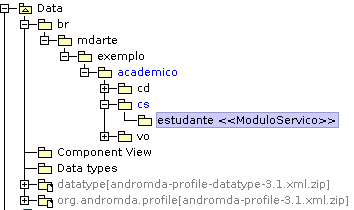
\includegraphics[width=200pt,height=200pt]{imgs/tutorial-mdarte-0008.png}
\end{figure} 
	
\item Crie um diagrama de classe dentro do pacote estudante, com o nome que desejar.
	
\item Crie uma classe com nome EstudanteHandler e estereótipo «Service». A classe EstudanteHandler deve ficar como na figura abaixo.
\begin{figure}[!htb]
	\centering
	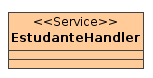
\includegraphics[width=150pt,height=120pt]{imgs/tutorial-mdarte-0009.png}
\end{figure} 
	
\item Crie uma classe com nome EstudanteException e estereótipo «ApplicationException».
\begin{figure}[!htb]
	\centering
	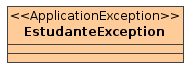
\includegraphics[width=150pt,height=120pt]{imgs/tutorial-mdarte-0010.png}
\end{figure}
	
\item Arraste para o diagrama de classes recém criado no pacote estudante a classe Estudante.
	
\item Crie uma relação de dependência entre as classes EstudanteHandler e Estudante, assim como entre EstudanteHandler e EstudanteException. Para isso, utilize a opção do MagicDraw ilustrada na figura abaixo. Clique na opção, depois clique na classe, ou método, de origem e arraste a seta até a classe destino.

\begin{figure}[!htb]
	\centering
	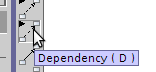
\includegraphics[width=110pt,height=90pt]{imgs/tutorial-mdarte-0012.png}
\end{figure}

\item Verifique se o diagrama está como a figura abaixo.
\begin{figure}[!htb]
	\centering
	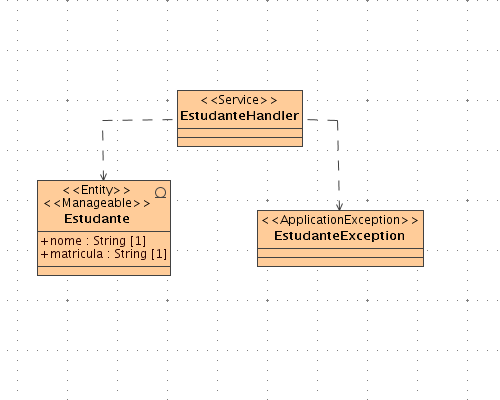
\includegraphics[width=300pt,height=350pt]{imgs/tutorial-mdarte-0011.png}
\end{figure}

\item A dependência entre EstudanteHandler e EstudanteException fará com que todos os métodos de EstudanteHandler possam lançar a exceção EstudanteException. Se a dependência tivesse sido entre algum método de EstudanteHandler e não com a própria classe, somente o método com dependência poderia lançar a exceção.

A dependência entre EstudanteHandler e Estudante cria os métodos de acesso ao banco na classe de serviço.

\item Agora faça o mesmo para criar um modulo de serviço para a classe Estudante.
	
\item No diretório da aplicação, execute o comando maven para validar o modelo e gerar as classes de serviço. O resultado apresentado deve ser “BUILD SUCCESSFULL”.
\end{enumerate}

\section{Implementando as classes de controle dos cruds gerados}

Nessa seção vamos implementar as classes de controle dos casos de uso gerados. Para isso, abriremos os arquivos <nomeCasoDeUso>ControleImpl.java. Esses arquivos são pontos de implementação onde deve ser concentrado todo o código que se queira adicionar manualmente às classes de controle. Como tais arquivos só são gerados caso ainda não existam, o código colocado neles não será sobrescrito, ao contrario do que ocorre se inserirmos manualmente codigo nos arquivos <nomeCasoDeUso>Controle.java .

De acordo com os casos de uso gerados automaticamente pelo gerador de cruds do MDArte, iremos implementar respectivamente os seguintes código nos seguintes arquivos, que devem portanto ser abertos no Eclipse ou em outra IDE desejada:

\begin{enumerate}
\item ConsultaEstudanteControleImpl.java :
\begin{lstlisting}[language=java]
public final void consultaEstudante(
	br.mdarte.exemplo.academico.web.geral.consultarEstudante.
	ConsultaEstudanteForm form, ViewContainer container
	) throws Exception {
    	
    Integer paginacao =
    	((Double)container.getAttribute(Constantes.PARAMETRO_PAGINA))
    	.intValue();
		
    EstudanteVO vo = new EstudanteVO();
    	
    vo.setNome(form.getNome());
    vo.setMatricula(form.getMatricula());
    	
    // nothing to be done for this operation, there are no properties that
    //can be set 
        
    Collection estudantes =
    	ServiceLocator.instance().getEstudanteHandlerBI()
    	.manipulaEstudante(new EstudanteImpl(), 
    	new FilterAction(vo, paginacao));
    	
    form.setEstudantes(estudantes);
}
\end{lstlisting}
		
\item MantemEstudanteControleImpl.java :
\begin{lstlisting}[language=java]
public final void carregaCurso(
	br.mdarte.exemplo.academico.web.geral.manterCurso.CarregaCursoForm 
	form, ViewContainer container) throws Exception {

    Curso c = new CursoImpl();
    	
    c.setId(form.getId());
    	
    c = (Curso)ServiceLocator.instance().getCursoHandlerBI()
    	.selectCurso(c).get(0);

    form.setNome(c.getNome());
    form.setId(c.getId());
    form.setCodigo(c.getCodigo());
    	
}
    	
public final void salvaCurso(
	br.mdarte.exemplo.academico.web.geral.manterCurso.SalvaCursoForm 
	form, ViewContainer container) throws Exception {

    Curso c = new CursoImpl();

	c.setId(form.getId());
	c.setCodigo(form.getCodigo()); 
	c.setNome(form.getNome());

	ServiceLocator.instance().getCursoHandlerBI()
		.insertOrUpdateCurso(c);
    	
}
\end{lstlisting}

\item DetalhaEstudanteControleImpl.java:
\begin{lstlisting}[language=java]
public final void carregaEstudante(
	br.mdarte.exemplo.academico.web.geral.detalharEstudante
	.CarregaEstudanteForm form, ViewContainer container) 
	throws Exception {
	
	Estudante e = new EstudanteImpl();
    	
   	e.setId(form.getId());
    	
   	e = (Estudante) ServiceLocator.instance().getEstudanteHandlerBI()
   		.selectEstudante(e).get(0);

   	form.setNome(e.getNome());
   	form.setId(e.getId());
   	form.setMatricula(e.getMatricula());
 	
}
\end{lstlisting}

\item ConsultaCursoControleImpl.java :
\begin{lstlisting}[language=java]
public final void consultaCurso(
	br.mdarte.exemplo.academico.web.geral.consultarCurso
	.ConsultaCursoForm form, ViewContainer container) 
	throws Exception {
    		
    Integer paginacao = 
    	((Double)container.getAttribute(Constantes.PARAMETRO_PAGINA))
    	.intValue();
    		
    CursoVO vo = new CursoVO();
    	
    vo.setNome(form.getNome());
    vo.setCodigo(form.getCodigo());
    	
    // nothing to be done for this operation, there are no properties 
    //that can be set
    Collection cursos = 
    	ServiceLocator.instance().getCursoHandlerBI().manipulaCurso(new
    	CursoImpl(), new FilterAction(vo, paginacao));
    	
    form.setCursos(cursos);	
}
\end{lstlisting}

\item MantemCursoControleImpl.java :
\begin{lstlisting}[language=java]
 public final void carregaCurso(
 	br.mdarte.exemplo.academico.web.geral.manterCurso
 	.CarregaCursoForm form, ViewContainer container) 
 	throws Exception {

   	Curso c = new CursoImpl();
    	
   	c.setId(form.getId());
    	
   	c = (Curso)ServiceLocator.instance().getCursoHandlerBI()
   		.selectCurso(c).get(0);
    	
   	form.setNome(c.getNome());
   	form.setId(c.getId());
   	form.setCodigo(c.getCodigo());
    	
}

public final void salvaCurso(
	br.mdarte.exemplo.academico.web.geral.manterCurso
	.SalvaCursoForm form, ViewContainer container)
	throws Exception {

   	Curso c = new CursoImpl();
    	
   	c.setId(form.getId());
    	
   	c = (Curso)ServiceLocator.instance().getCursoHandlerBI()
   		.selectCurso(c).get(0);
    	
	c.setCodigo(form.getCodigo()); 
	c.setNome(form.getNome());

	ServiceLocator.instance().getCursoHandlerBI().insertOrUpdateCurso(c);
}
\end{lstlisting}

\item DetalhaCursoControleImpl.java :
\begin{lstlisting}
public final void carregaCurso(br.mdarte.exemplo.academico.web.geral.detalharCurso.CarregaCursoForm form, ViewContainer container) throws Exception {
	Curso c = new CursoImpl();
    	
    c.setId(form.getId());
    	
    c = (Curso)ServiceLocator.instance().getCursoHandlerBI().selectCurso(c).get(0);

    form.setNome(c.getNome());
    form.setId(c.getId());
    form.setCodigo(c.getCodigo());	
}
\end{lstlisting}
\end{enumerate}

Agora, no terminal, no <DiretorioProjeto> executaremos o seguinte comando :

\begin{lstlisting}[language=bash]
maven compile deploy
\end{lstlisting}

Abriremos agora o eclipse, daremos Start no servidor jboss e verificaremos então no navegador o resultado do nosso sistema.